\begin{tikzpicture}
	\node[anchor=south west, inner sep=0] (image) at (0,0) {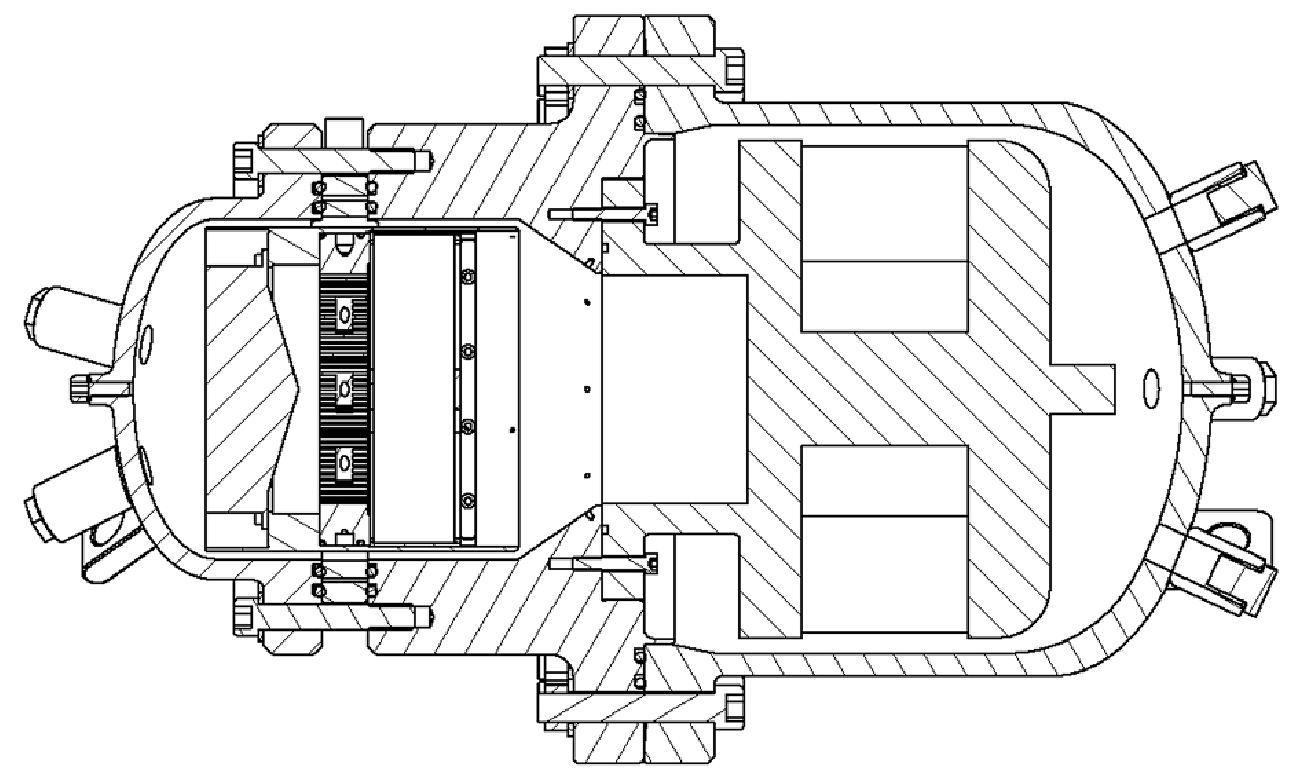
\includegraphics[angle=0,origin=c,width=.6\textwidth]{../fig/fig_TACOTSchematics/TACOT.png}};
	
	\begin{scope}[x={(image.south east)},y={(image.north west)}]
	
%		\filldraw (0,0) circle (2pt); 
%		\filldraw[green] (1,0) circle (1pt);
%		\filldraw[red] (1,1) circle (1pt);		
%		\filldraw[blue] (0,1) circle (1pt);
%		\draw[help lines,xstep=.1,ystep=.1] (0,0) grid (1,1);
%		\fill[orange, rounded corners, opacity=1,draw=orange] (.46,.65) -- ++(132:.09) -- ++(0,-.44) -- ++(48:.09) -- cycle;
		\draw[MatlabYellow,rounded corners,very thick,preaction={fill=MatlabYellow!20,opacity=.5}] (.46,.65) -- ++(132:.09) -- ++(-.03,0) -- ++(0,-.44) --++(.03,0) -- ++(48:.09) -- cycle; %node[left,pos=.5,label={[rotate=90]center:Cavité}]{};
		\draw[MatlabYellow] (.415,0.5) node [label={[rotate=90]center:\shortstack{\textbf{Volume}\\\textbf{d'adaptation}}}]{};
		
%		\draw[blue] (.5,.5) node [anchor=center, preaction={fill=black!20,opacity=.7}] {RIX};
%		\draw[red] (.33,.5) node [anchor=center, preaction={fill=black!20,opacity=.7}] {TA core};	
	
		\draw[MatlabOrange,rounded corners,very thick,preaction={fill=MatlabOrange!20,opacity=.5}] (.365,.7) rectangle (.245,.3) node[pos=.5,label={[rotate=90]center:\small \textbf{Noyau TA}}]{};
		
		\node (AHX) at (.27,.65) {};
		\node (Reg) at (.32,.65) {};
		\node (CHX) at (.36,.65) {};
		\node (RIX) at (.77,.4) {};
		\node (HP) at (.19,.4) {};
		
		\draw[<-,very thick,MatlabOrange] (AHX.center) to[out=90,in=180] ($(AHX)+(-.15,.7)$) node[right]{\'Echangeur de chaleur ambiant};		
		\draw[<-,very thick] (Reg.center) to[out=90,in=180] ($(Reg)+(0,.6)$) node[right]{Régénérateur};
		\draw[<-,very thick,MatlabBlue] (CHX.center) to[out=90,in=180] ($(CHX)+(.15,.5)$) node[right]{\'Echangeur de chaleur froid};
		
		\draw[->,very thick,green!50!black] ($(RIX)+(0,-.5)$) -- (RIX.center) node[pos=0,anchor=north]{Source acoustique principale};
		\draw[->,very thick,green!50!black] ($(HP)+(0,-.5)$) -- (HP.center) node[pos=0,anchor=north]{Source acoustique secondaire};
		
%		\draw [white] (.455,.5) node{+};
%		\draw [white] (.41,.65) node{+};
%		\draw [white] (.41,.5) node{+};
%		\draw [white] (.41,.35) node{+};

	\end{scope}

	
\end{tikzpicture}